\documentclass[a4paper,10pt,openright,openbib,twocolumn]{article}
%\usepackage[portuges]{babel}
\usepackage[T1]{fontenc}
\usepackage{ae}
\usepackage[utf8]{inputenc}
\usepackage[pdftex]{graphicx}
\usepackage{url}
\usepackage{listings}
\usepackage{verbatim}
\usepackage{enumerate}
\usepackage[pdftex, bookmarks, colorlinks, linkcolor=black, urlcolor=blue]{hyperref} 
%\usepackage[a4paper,left=2.5cm,right=2.5cm,top=3.5cm,bottom=3.5cm]{geometry}
\usepackage[paper=a4paper,top=2cm,left=2cm,right=1.5cm,bottom=2cm,foot=1cm]{geometry}
\usepackage{colortbl}
\usepackage[margin=10pt,font=small,labelfont=bf]{caption}
\usepackage{mdwlist}
\usepackage{cleveref}
\usepackage{epsfig}

\usepackage{multicol}
\usepackage{appendix}
\usepackage{listings}
\usepackage{float}



\setlength{\parindent}{0cm}
\setlength{\parskip}{2pt}

\lstset{ %
language=C++,                % choose the language of the code
basicstyle=\scriptsize,       % the size of the fonts that are used for the code
numberstyle=\scriptsize,      % the size of the fonts that are used for the line-numbers
stepnumber=1,                   % the step between two line-numbers. If it is 1 each line will be numbered
numbersep=5pt,                  % how far the line-numbers are from the code
showspaces=false,               % show spaces adding particular underscores
showstringspaces=false,         % underline spaces within strings
showtabs=false,                 % show tabs within strings adding particular underscores
tabsize=2,          % sets default tabsize to 2 spaces
captionpos=b,           % sets the caption-position to bottom
breaklines=true,        % sets automatic line breaking
breakatwhitespace=false,    % sets if automatic breaks should only happen at whitespace
}


\begin{document}
\title{The Cilk Plus Extension}
\date{\today}
\begin{multicols}{2}
\author{
    Brito, Rui\\
    PG22781\\
    Department of Informatics\\
    University of Minho\\
    ruibrito666@gmail.com
  \and
    Alves, José\\
    PG22765\\
    Department of Informatics\\
    University of Minho\\
    zealves.080@gmail.com
}
\date{}
\maketitle
\end{multicols}

\begin{abstract}
    This report presents an analysis of the Cilk Plus extension for the C and C++ languages. Cilk Plus is not just a library, it is an extension implemented by the compiler and the Cilk Plus runtime, thus allowing for lower overhead than some of it's competitors. We compare Cilk Plus with a very well known alternative, OpenMP, and, although some results were positive (namely, recursive algorithms), overall, OpenMP wins. 
\end{abstract}

\section{Introduction}   
    Cilk Plus provides an easy way to exploit parallelism inside an application, by using only three keywords, one can fully take advantage of both multicore and SIMD extensions. In \Cref{cilk} an introduction on what Cilk Plus is is given while \Cref{key} introduces its main features. \Cref{extension} details what the language adds to parallel programming paradigms and provides some examples. \Cref{openmp} explains how Cilk fairs against OpenMp. \Cref{conc} states Cilk Plus' advantages and disadvantages.


\section{What is Cilk Plus} \label{cilk}
Intel Cilk is an extension to the C and C++ languages to support task and data parallelism. Unlike most of it's competitors, Cilk Plus is not just a library, it is a language extension that is implemented by the compiler and the Cilk Plus runtime, allowing lower overhead than library-only solutions. Cilk Plus is developed by Intel, and thus, through the Intel runtime, supports composability. Many applications are composed of independently written components. Typically, the components communicate with each other through higher-level interfaces rather than at a lower, implementation-oriented level. To allow that level of collaboration in a parallel program, the task scheduler has to allow composability (that is, when modules are combined to form the application, they continue to work and perform well). Cilk Plus achieves this with a work-stealing task scheduler.


\section{Key Features} \label{key}

The main key features of Cilk Plus are as follows:
\begin{itemize}
    \item Keywords: cilk adds three new keywords to the C/C++ languages to better express task parallelism in an application;
    \item Reducers: a mechanism to eliminate contention for shared variables;
    \item \#pragma simd: a directive that tells the compiler a loop should be vectorized;
    \item Array Notations: a language addition to specify data paralellism for arrays or sections of arrays;
\end{itemize}


\section{The Cilk Plus Extension} \label{extension}

As seen in previous section, Cilk Plus as several of expressing parallelism, the following subsections will provide some insight into some of its core features and how it works.

\subsection {Keywords} 
The are only three keywords in the Cilk Plus extensions and they provide a simple yet powerful way of expressing parallelism, they are as follows:
\begin{itemize}
    \item cilk\_spawn: tells the runtime environment that the statement following the cilk\_spawn keyword can be run in parallel with other statements;
    \item cilk\_sync: tells the runtime environment that all children of the spawning block must finish their execution before execution can continue;
    \item cilk\_for: a replacement for the standard C/C++ for loop that lets iterations run in parallel; 
\end{itemize}
The following example shows the typical use of the cilk\_spawn and cilk\_sync keywords:
\begin{minipage}{.45\textwidth}
    \begin{lstlisting}[caption=Computation of the nth Fibonacci Number using Cilk Plus]
        double fib(double n) {
            if (n < 2)
                return n;

            if (n < 30)
                return seq_fib(n);

            double x = cilk_spawn fib(n-1);
            double y = fib(n-2);
            cilk_sync;
            return x + y;
        }
    \end{lstlisting}
\end{minipage}

The following example shows the use of the cilk\_for keyword:

\begin{minipage}{.45\textwidth}
\begin{lstlisting}[caption=Matrix multiplication using Cilk Plus]
float* matrixDot (float *a, float *b, int n) {
    
    float value = 0;
    float *res = (float*) malloc(n * n * sizeof(float));

    cilk_for (int i = 0; i < n; ++i) {
        for(int j = 0; j < n; ++j) {            
            for(int k = 0; k < n; ++k) {
                    value += a[i * n + k] * b[k * n + j];
            }
            res[i * n + j] = value;
            value = 0;
        }
    }
    
    
    return res;
}
\end{lstlisting}    
\end{minipage}

\subsubsection{More on cilk\_for}
A call to cilk\_for isn't the same as spawning each iteration of the loop. What actually happens is, the compiler converts the loop body to a function that is called recursively using a divide-and-conquer strategy. \\
    \begin{figure}[!htb]
            \centering
            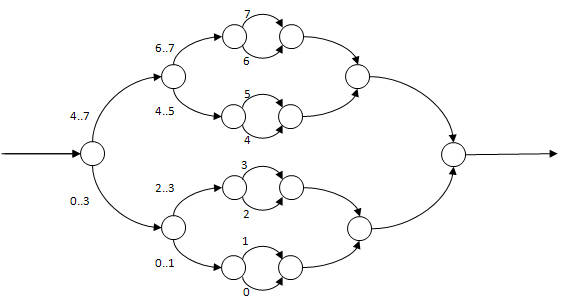
\includegraphics[scale=0.9]{../pres/images/cilkfor.jpg}
            \caption{cilk\_for with N=8 iterations}
            \label{roofline}
        \end{figure}
        
As it can be seen in the previous figure, the worker whose execution reached the cilk\_for construct computes the trip count, it then takes the upper half of the iterations and puts it in its own work queue for later evaluation. It then continues to divide and conquer the lower trip count, until the trip count becomes sufficiently small (determined heuristically at run time). It then executes the iterations sequentially. Upon completion, the worker pops the next work item, which was posted last, from its own work queue. This will be the second set of iteration of the lower half. If another worker has an empty work queue, it might steal work from the core that created the list of work items corresponding to the loop iterations. This is how concurrent work is created in Cilk Plus.

\subsection{Reducers}

Reducers allow thread-safe access to shared objects by giving each parallel strand a separate instance of the object, called a view. The Cilk Plus Reducers are as follows:
        \begin{itemize}
            \item reducer\_list\_append: Creates a list by adding elements to the back;
            \item reducer\_list\_prepend: Creates a list by adding elements to the front;
            \item reducer\_max: Calculates the maximum value of a set of values;
            \item reducer\_max\_index: Calculates the maximum value and index of that value of a set of values;
            \item reducer\_min: Calculates the minimum value of a set of values;
            \item reducer\_min\_index: Calculates the minimum value and index of that value of a set of values;
            \item reducer\_opadd: Calculates the sum of a set of values;
            \item reducer\_opand: Calculates the binary AND of a set of values;
            \item reducer\_opor: Calculate the binary OR of a set of values;
            \item reducer\_opxor: Calculate the binary XOR of a set of values;
            \item reducer\_string: Accumulates a string using append operations;
            \item reducer\_wstring: Accumulates a "wide" string using append operations;
            \item reducer\_ostream: An output stream that can be written in parallel;
            \item reducer\_ostream: An output stream that can be written in parallel;
        \end{itemize}

A small usage example follows:\\

\begin{minipage}{.45\textwidth}    
        \begin{lstlisting}[caption=Example showing the usage of Cilk Plus Reducers]
    void reducer_list_test() {
        cilk::reducer_list_append<char> letters_reducer;

        cilk_for(char ch = 'a'; ch <= 'z'; ch++){
            simulated_work();
            letters_reducer.push_back(ch);
        }

        const std::list<char> &letters = letters_reducer.get_value();

        for(std::list<char>::const_iterator i = letters.begin(); i != letters.end(); i++) {
            std::cout << " " << *i;
        }
        std::cout << std::endl;
    }
        \end{lstlisting}
\end{minipage}

\subsection{Array Notation}

Array notation is intended to allow users to directly express high level parallel vector array operations in their code. This assists the compiler in performing vectorization and auto-parallelization. More predictable vectorization, improved performance and better hardware resource utilization are key goals. 

This is a direct extension to the C/C++ languages. Here is an example:

\begin{minipage}{.45\textwidth}    
        \begin{lstlisting}[caption=Examples of Cilk Plus Array Notation]
// Copy elements 10->19 in A to elements 0->9 in B.
B[0:10] = A[10:10];
// Transpose row 0, columns 0-9 of A, into column 0, rows 0-9 of B.
B[0:10][0] = A[0][0:10];
// Copy the specified array section in the 2nd and 3rd dimensions of A into the 1st and 4th dimensions of B.
B[0:10][0][0][0:5] = A[3][0:10][0:5][5]
// Set all elements of A to 1.0.
A[:] = 1.0;
// Add elements 10->19 from A with elements 0->9 from B and place in elements 20->29 in C.
C[20:10] = A[10:10] + B[0:10];
// Element-wise equality test of B and C, resulting in an array of Boolean values, which are placed in A.
A[:] = B[:] == C[:];
        \end{lstlisting}
\end{minipage}

\subsection{The Cilk Plus Scheduler}
The Cilk Plus runtime uses a work-stealing scheduler to dynamically load-balance the tasks that are created by a Cilk Plus program. In abstract, the runtime uses worker threads. Each of these worker threads manipulates a stack, by removing task at the bottom. When a worker thread as an empty stack, it steals a task from the top of another worker thread's stack. If the flow of the program reaches a cilk\_sync construct, then it tries to keep busy by popping tasks from the tail of its stack.

\section{Cilk vs. OpenMP} \label{openmp}
\subsection{Test Environment}

In order to achieve precise and consistent results, all tests were run on a dedicated execution of the algorithm, with niceness set to -20, to ensure the tests execution was top priority to the OS's scheduler. Furthermore, all network connections were disabled. To decrease the chance of human error, all tests were hard-coded into a bash script, with another script traversing those tests and showing the results. Also, it should be noted that every test was run at least 3 times. A 5\% error margin was checked between execution (the aforementioned script handles this part), and if this margin is not met, the tests are run again. It should also be noted that due to the nature of Cilk Plus the compiler used was icc (13.0.2).

\begin{center}                 
\begin{table}[!hc]
            \begin{tabular}{|c|c|}            
            \hline
              & MacBookPro\\
            & Intel Ivy-Bridge i7\\
            \hline
            \# processors & 1\\
            \# cores per processor & 4\\
            hyper-threading & yes\\
            clock frequency(GHz) & 2.3\\
            L1 size & 64KB\\
            L2 size & 256KB\\
            L3 size & 6MB\\
            RAM size & 16GB\\
            \hline                                
            \end{tabular}
            \caption{Test Machine}
    \end{table}
        \end{center}

\footnotesize
Note: no tests were run on search because of problems with the icc licence.
\normalsize


\subsection{Results}

        \begin{figure}[H]
            \centering
            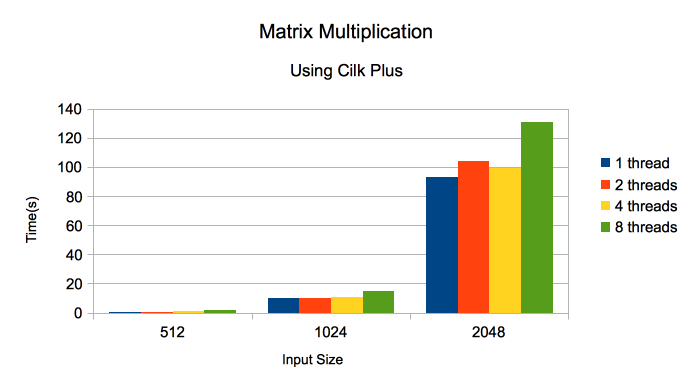
\includegraphics[scale=0.45]{images/matmultcilk.png}
            \caption{Results for matrix multiplication using Cilk Plus}
            \label{roofline}
        \end{figure}
        \begin{figure}[H]
            \centering
            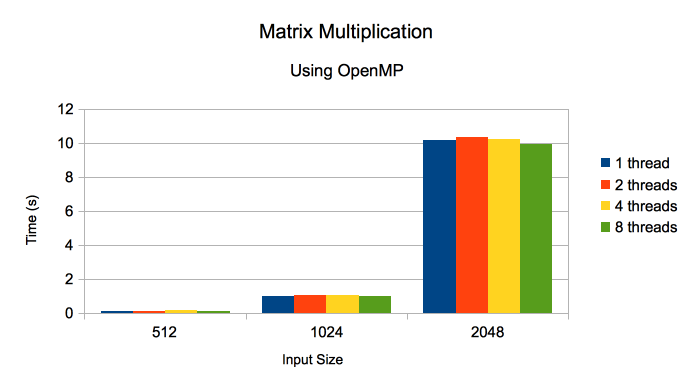
\includegraphics[scale=0.45]{images/matmultopenmp.png}
            \caption{Results for matrix multiplication using OpenMP}
            \label{roofline}
        \end{figure}
        As can be seen in the results above, Matrix Multiplication performs better in the OpenMP implementation, this is probably due to the way the cache is used.\\

        \begin{figure}[H]
            \centering
            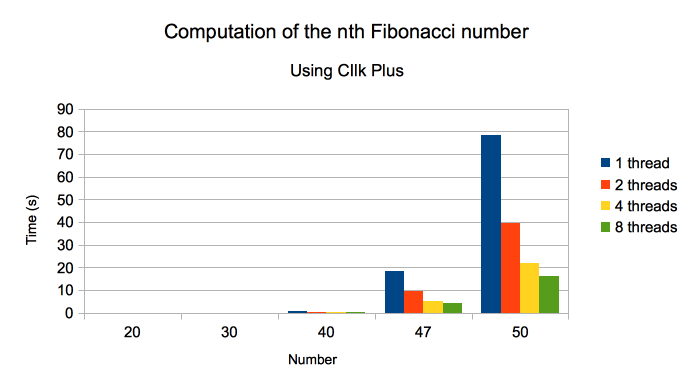
\includegraphics[scale=0.45]{images/fibcilk.png}
            \caption{Results for fibonacci computation using Cilk Plus}
            \label{roofline}
        \end{figure}
        \begin{figure}[H]
            \centering
            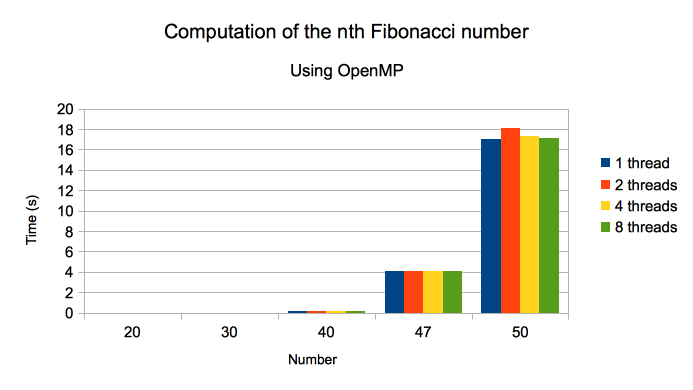
\includegraphics[scale=0.45]{images/fibopenmp.png}
            \caption{Results for fibonacci computation using OpenMP}
            \label{roofline}
        \end{figure}
        Fibonacci is a recursive algorithm and so it was expected for it to perform better in the Cilk Plus implementation, and it did. OpenMP's performance is very linear, while the Cilk Plus version scales much better. This is because of the work-stealing mechanism. \\

        \begin{figure}[H]
            \centering
            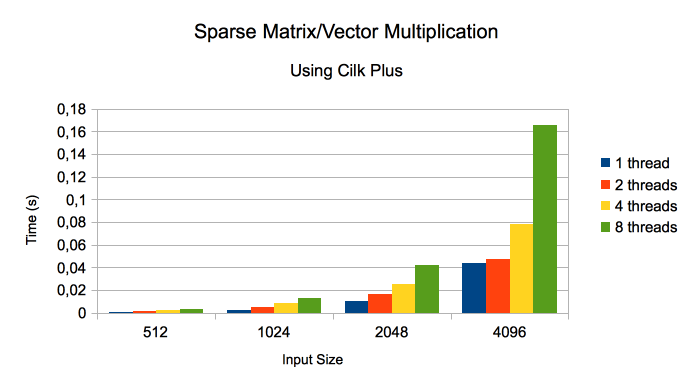
\includegraphics[scale=0.45]{images/matvectcilk.png}
            \caption{Results for sparse matrix/vector multiplication using Cilk Plus}
            \label{roofline}
        \end{figure}
        \begin{figure}[H]
            \centering
            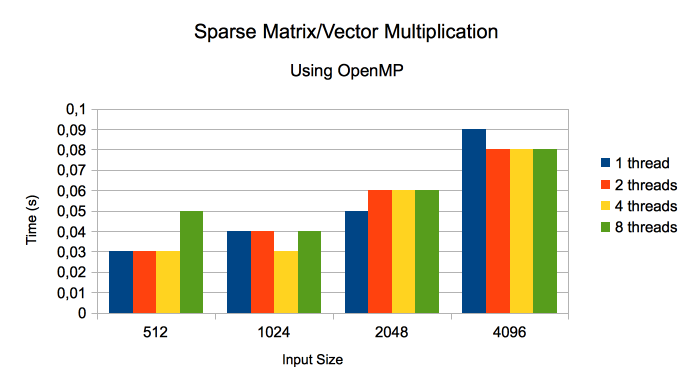
\includegraphics[scale=0.45]{images/matvectopenmp.png}
            \caption{Results for sparse matrix/vector multiplication using OpenMP}
            \label{roofline}
        \end{figure}
        Sparse Matrix/Vector multiplication was overall better in the Cilk implementation but not when the size of the matrix was 4096x4096. This is probably to cache alignment issues or because the problem doesn't fit in cache altogether, since each thread needs a stack and that stack, most probably, is in cache. \\

        \begin{figure}[H]
            \centering
            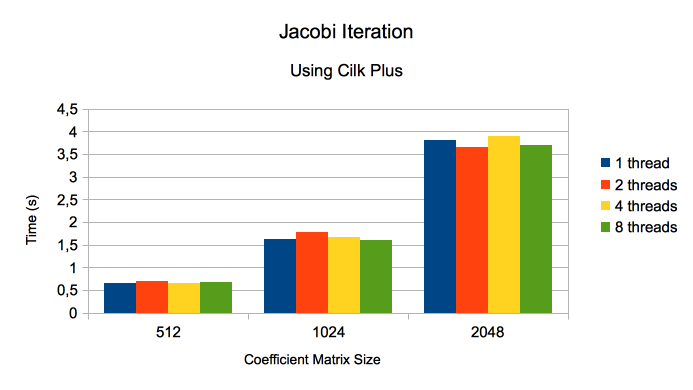
\includegraphics[scale=0.45]{images/jacobicilk.png}
            \caption{Results for jacobi iteration using Cilk Plus}
            \label{roofline}
        \end{figure}
        \begin{figure}[H]
            \centering
            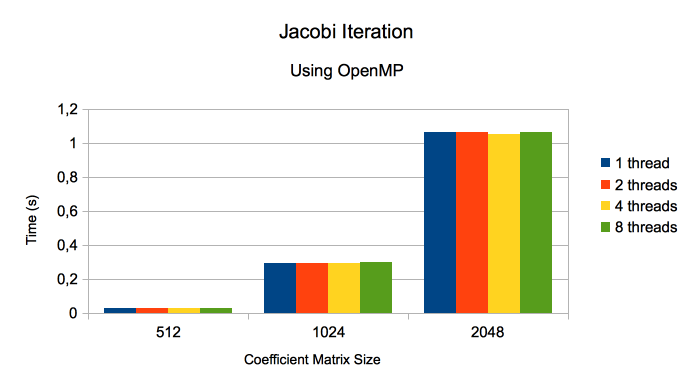
\includegraphics[scale=0.45]{images/jacobiopenmp.png}
            \caption{Results for jacobi iteration using OpenMP}
            \label{roofline}
        \end{figure}
        Jacobi also performed better with openMP, this is mostly, we believe, due to high synchronization between worker threads. \\

\section{Conclusion} \label{conc}

Ease of use if definitely an advantage over Cilk Plus competitors. Although it is not as fine grained as OpenMP, the Intel runtime allows for it to be used with other tools, such as TBB (composability). We found it is good for recursive algorithms, or algorithms that can be divided in tasks. Automatic load balancing is one of the best things about Cilk Plus, in fact, Intel goes as far as claiming, guaranteed maximum memory usage scaling. It simplifies adding parallelism to existing serial programs. Multiple attributes of the extensions support this, including the non intrusive syntax, the ability to easily revert back to the serial program, the guarantee of serial semantics equivalence, and the low overhead of spawning a task.

\end{document}
